\documentclass[12pt,a4paper]{report}

\usepackage[utf8]{inputenc} % pentru suport diacritice
\usepackage[romanian]{babel} % setări pentru limba română 
\renewcommand\familydefault{\sfdefault} % sans serif

\usepackage[margin=2.54cm]{geometry}	% dimensiuni pagină și margini
\usepackage{graphicx} % support the \includegraphics command and options

% formatting sections and subsections
\usepackage{textcase}
\usepackage{titlesec}
\titleformat{\chapter}{\large\bfseries\MakeUppercase}{\thechapter}{2ex}{}[\vspace*{-1.5cm}]
\titleformat*{\section}{\large\bfseries}
\titleformat*{\subsection}{\large\bfseries}
\titleformat*{\subsubsection}{\large\bfseries}

\usepackage{chngcntr}
\counterwithout{figure}{chapter} % no chapter number in figure labels
\counterwithout{table}{chapter} % no chapter number in table labels
\counterwithout{equation}{chapter} % no chapter number in equation labels

\usepackage{booktabs} % for much better looking tables
\usepackage{url} % Useful for inserting web links nicely
\usepackage[bookmarks,unicode,hidelinks]{hyperref}

\usepackage{array} % for better arrays (eg matrices) in maths
\usepackage{paralist} % very flexible & customisable lists (eg. enumerate/itemize, etc.)
\usepackage{verbatim} % adds environment for commenting out blocks of text & for better verbatim
\usepackage{subfig} % make it possible to include more than one captioned figure/table in a single float
\usepackage{enumitem}
\setlist{noitemsep}

%%% HEADERS & FOOTERS
\usepackage{fancyhdr}
\pagestyle{empty}
\renewcommand{\headrulewidth}{0pt}
\renewcommand{\footrulewidth}{0pt}
\lhead{}\chead{}\rhead{}
\lfoot{}\cfoot{\thepage}\rfoot{}

\newenvironment{conditions}
  {\par\vspace{\abovedisplayskip}\noindent\begin{tabular}{>{$}l<{$} @{${}={}$} l}}
  {\end{tabular}\par\vspace{\belowdisplayskip}}

\newcommand{\HeaderLineSpace}{-0.5cm}
\newcommand{\UniTextRO}{UNIVERSITATEA POLITEHNICA DIN BUCUREȘTI \\[\HeaderLineSpace] 
FACULTATEA DE AUTOMATICĂ ȘI CALCULATOARE \\[\HeaderLineSpace]
DEPARTAMENTUL CALCULATOARE\\}
\newcommand{\DiplomaRO}{PROIECT DE DIPLOMĂ}
\newcommand{\AdvisorRO}{Coordonator științific:}
\newcommand{\BucRO}{BUCUREȘTI}

\newcommand{\UniTextEN}{UNIVERSITY POLITEHNICA OF BUCHAREST \\[\HeaderLineSpace]
FACULTY OF AUTOMATIC CONTROL AND COMPUTERS \\[\HeaderLineSpace]
COMPUTER SCIENCE DEPARTMENT\\}
\newcommand{\DiplomaEN}{DIPLOMA PROJECT}
\newcommand{\AdvisorEN}{Thesis advisor:}
\newcommand{\BucEN}{BUCHAREST}

\newcommand{\frontPage}[6]{
\begin{titlepage}
\begin{center}
{\Large #1}  % header (university, faculty, department)
\vspace{50pt}
\begin{tabular}{p{6cm}p{4cm}}

\includegraphics[scale=0.8]{pics/upb-logo.jpg} &
	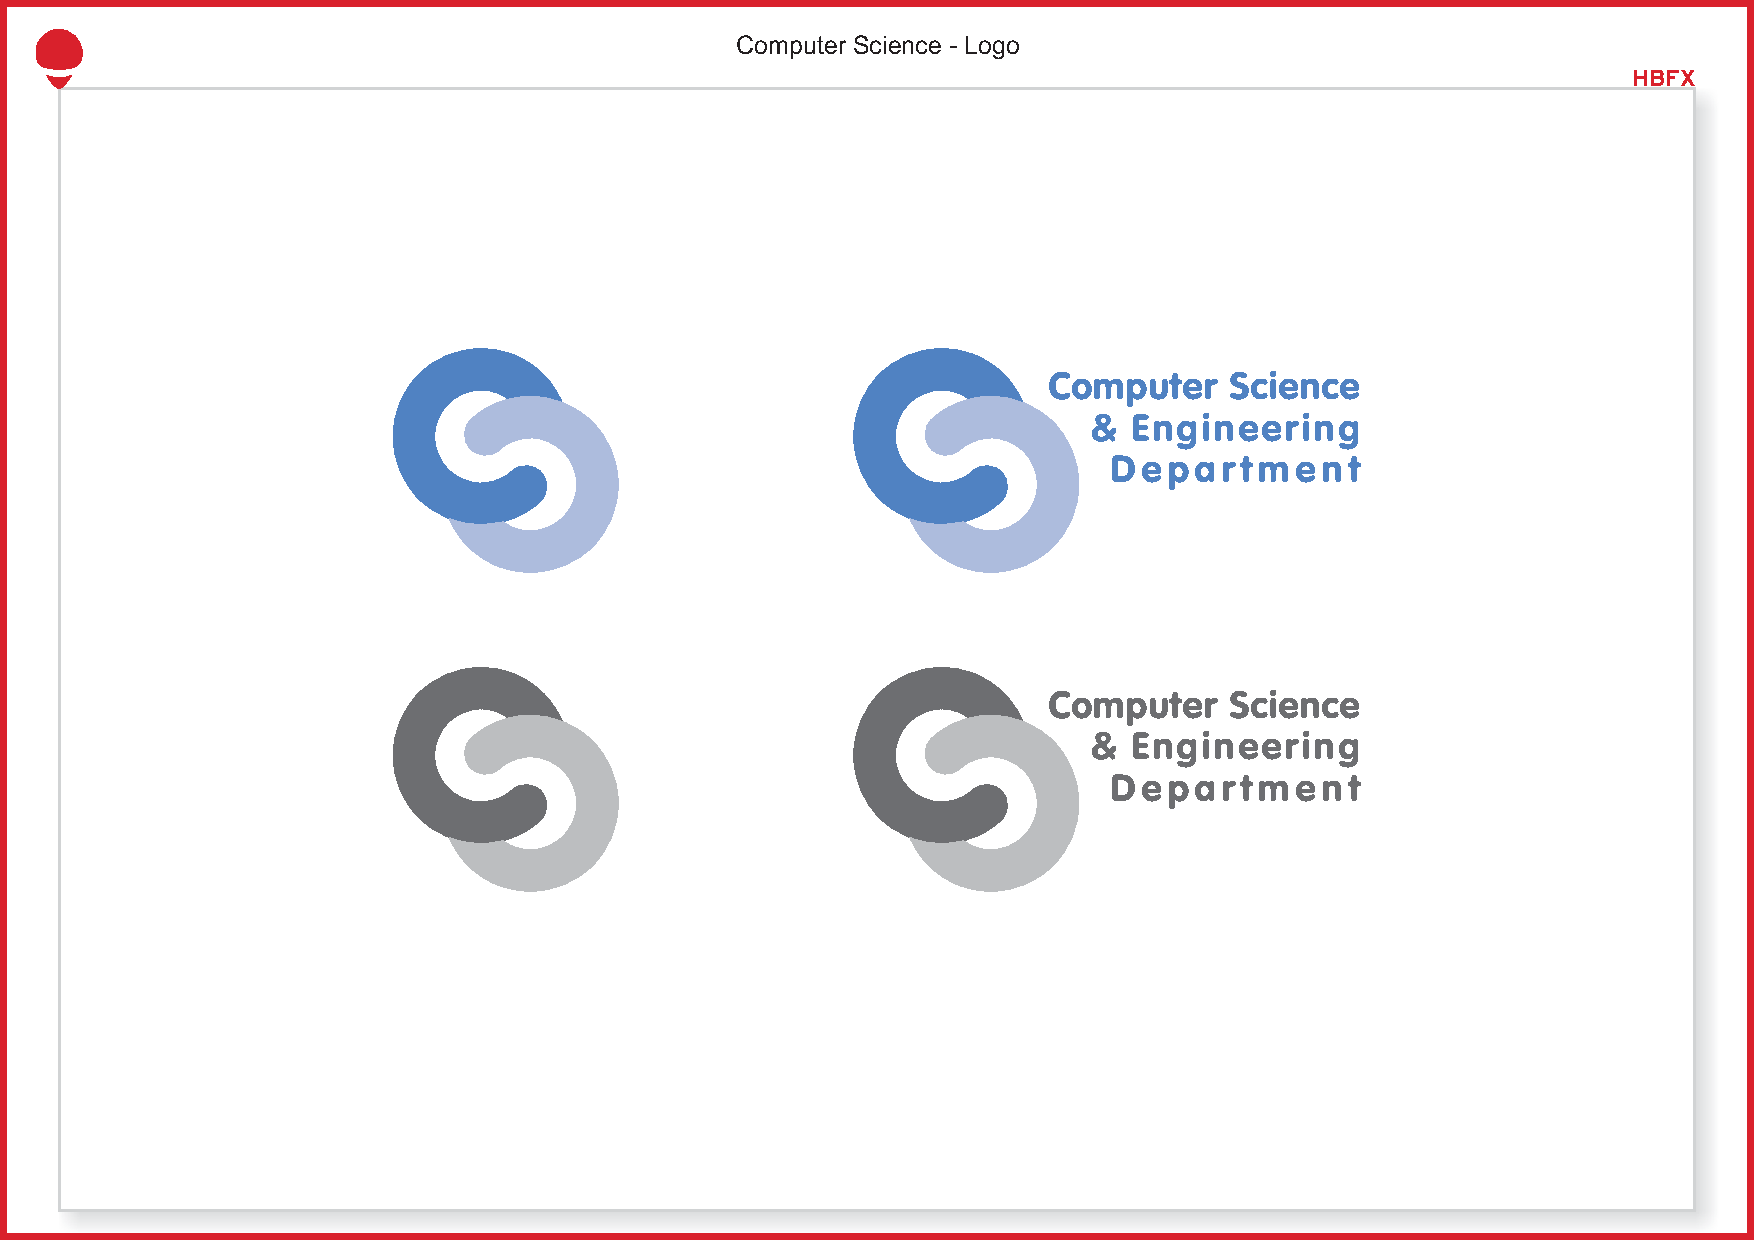
\includegraphics[scale=0.5,trim={14cm 11cm 2cm 5cm},clip=true]{pics/cs-logo.pdf}
\end{tabular}

\vspace{105pt}
{\Huge #2}\\                           % diploma project text
\vspace{40pt}
{\Large #3}\\ \vspace{0pt}  % project title
{\Large #4}\\                          % project subtitle
\vspace{40pt}
{\LARGE \Name}\\                   % student name
\end{center}
\vspace{60pt}
\begin{tabular*}{\textwidth}{@{\extracolsep{\fill}}p{6cm}r}
&{\large\textbf{#5}}\vspace{10pt}\\      % scientific advisor
&{\large \Advisor}                                    % advisor name
\end{tabular*}
\vspace{20pt}
\begin{center}
{\large\textbf{#6}}\\                                % bucharest
\vspace{0pt}
{\normalsize \Year}
\end{center}
\end{titlepage}
}

\newcommand{\frontPageRO}{\frontPage{\UniTextRO}{\DiplomaRO}{\ProjectTitleRO}{\ProjectSubtitleRO}{\AdvisorRO}{\BucRO}}
\newcommand{\frontPageEN}{\frontPage{\UniTextEN}{\DiplomaEN}{\ProjectTitleEN}{\ProjectSubtitleEN}{\AdvisorEN}{\BucEN}}

\linespread{1.5}
\setlength\parindent{0pt}
\setlength\parskip{.28cm}

%% Abstract macro
\newcommand{\AbstractPage}{
\begin{titlepage}
\textbf{\large SINOPSIS}\par
\AbstractRO\par\vfill
\textbf{\large ABSTRACT}\par
\AbstractEN \vfill
\end{titlepage}
}

%% Thank you macro
\newcommand{\ThanksPage}{
\begin{titlepage}
{\noindent \large\textbf{MULȚUMIRI}}\\
\Thanks
\end{titlepage}
}



%%%%%%%%%%%%%%%%%%%%%%%%%%%%%%%%%%%%%%%%%%%%%%%%%%   
%%
%%          End of template definitions
%%   
%%%%%%%%%%%%%%%%%%%%%%%%%%%%%%%%%%%%%%%%%%%%%%%%%%


%%% Puteți elimina aceste linii din lucrare, servesc numai pentru template.
\newcommand{\worktype}[1]{[\textit{#1}] }
\newcommand{\dezvoltare}{\worktype{Dezvoltare de produs}}
\newcommand{\cercetare}{\worktype{Cercetare}}
\newcommand{\ambele}{\worktype{Ambele}}
%%%


%%
%%   Campurile de mai jos trebuie modificate de autor. Modificati doar continutul, nu si numele fiecarei definitii
%%
\newcommand{\ProjectTitleRO}{Titlul proiectului de diplomă (ex: Șablon proiect de diplomă)}
\newcommand{\ProjectSubtitleRO}{Subtitlu (ex: versiunea 2018)}
\newcommand{\ProjectTitleEN}{Diploma Project Title  (eg: Diploma project template)}
\newcommand{\ProjectSubtitleEN}{Subtitle (eg: 2018 version)}
\newcommand{\Name}{Ioana Popescu}
\newcommand{\Advisor}{Prof. dr. ing. Andrei Ionescu}
\newcommand{\Year}{2018}

% Setări document
\title{Proiect de diplomă}
\author{\Name}
\date{\Year}

%%
%%   Campurile aferente rezumatului
%%
\newcommand{\AbstractRO}{Sinopsisul proiectului are rol de introducere, conținând atât o descriere pe scurt a problemei abordate cât și o enumerare sumară a rezultatelor și a concluziilor. Se recomandă ca sinopsisul să fie redactat într-un limbaj accesibil unei persoane nefamiliarizate cu domeniul, dar în același timp destul de specific pentru a oferi rapid o vedere de ansamblu asupra proiectului prezentat.
Sinopsisul proiectului va fi redactat atât în română cât și în engleză. Ca dimensiunea recomandată aceasta secțiune va avea maxim 200 de cuvinte pentru fiecare variantă. Împreună, ambele variante se vor încadra într-o singură pagină.}

\newcommand{\AbstractEN}{The abstract has an introductory role and should engulf both a brief description of the issue at hand, as well as an overview of the obtained results and conclusions. The abstract should be formulated such that even somebody that is unfamiliar with the projects’ domain can grasp the objectives of the thesis while, at the same time, retaining a specificity level offering a bird’s eye view of the project.
The projects’ abstract will be elaborated in both Romanian and English. The recommended size for this section is limited to 200 words for each version. Together, both versions will fit in one page.}

%%
%%   Campurile aferente paginii de multumiri
%%
\newcommand{\Thanks}{(opțional) Aici puteți introduce o secțiunea specială de mulțumiri / acknowledgments. }

\begin{document}

\frontPageRO
\frontPageEN

\begingroup
\linespread{1}
\tableofcontents
\endgroup

\AbstractPage

% poate fi comentata sau stearsa
\ThanksPage


% Textul licentei incepe de aici 



\chapter{Introducere}\pagestyle{fancy}
% * <marios.choudary@gmail.com> 2018-02-28T11:38:18.106Z:
% 
% > INTRODUCERE
% Am scos de aici referintele la font pentru a nu mai fi dependenti de Calibri. Personal, nici nu sunt sigur ca ajuta prea mult aceasta recomandare si mi se pare bun font-ul default din Latex (Computer Modern). Daca sunteti de-acord, va rog sa stergeti liniile comentate de mai jos, precum si cele referitoare la fontul Calibri din restul documentului.
% 
% ^.
Parametrii de formatare recomandați pentru lucrare: 
\begin{itemize}
 %\item Font recomandat: Calibri; Dimensiune font: 12; 
 \item Dimensiune font: 12; 
 \item Spațiere între linii: 1,5; Spațiere după paragraf: 8pt;
 \item Stil: Justified;
 \item Dimensiune pagină: A4; Margini: 2,54cm/ 2,54cm/ 2,54cm/ 2,54cm;
 %\item Heading1: Calibri, 14, bold, all caps;
 %\item Heading2: Calibri, 14, bold;
 %\item Heading3: Calibri, 12. 
 %\item Font pentru formule: Cambria Math, 12.
 \item Heading1: 14, bold, all caps;
 \item Heading2: 14, bold;
 \item Heading3: 12. 
 \item Font size pentru formule: 12.
\end{itemize}
În cadrul introducerii, este necesară abordarea următoarelor puncte care reprezintă de fapt familiarizarea cititorului (comisia, alți colegi sau experți în domeniu) cu tema proiectului, soluția propusa și cuprinsul/structura lucrării. Deși introducerea poate conține și unele elemente mai generale, se recomandă păstrarea unui limbaj tehnic, specific audienței care va citi lucrarea.

În cadrul capitolelor următoare, veți regăsi o serie notații de forma \dezvoltare, \cercetare. Acest tip de formatare este utilizat exclusiv în acest template pentru a marca sfaturi și cerințe specifice pentru lucrări de diploma cu specific diferit. În pregătirea documentului vostru, nu veți utiliza aceste marcaje. 
Elementele pe care trebuie să le abordați în introducere sunt descrise în cadrul subcapitolelor de mai jos. 
\section{Context}
O scurtă introducere a proiectului, motivație, explicație de ce este relevant domeniul proiectului.
\section{Problema} 
Care este problema pe care proiectul o va rezolva.
\section{Obiective}
Care sunt obiectivele proiectului/soluției/abordării/ideii; Ce creșteri sau evoluții determină rezolvarea proiectului.
\section{Soluția propusă} 
Descrierea pe scurt a soluției implementate; ce abordare este propusă (nu detalierea utilitarelor și a tehnologiilor, ci abordarea și ideea propusă de către autor).
\section{Rezultatele obținute}
Descriere pe scurt a rezultatelor obținute, eventual de ce acestea sunt importante față de alte soluții sau studii.
\section{Structura lucrării}
Un paragraf în care fiecare dintre secțiunile următoare este prezentată în 1-2 fraze, punând accentul pe elementele cele mai semnificative din fiecare secțiune.



\chapter{Analiza Cerințelor / Motivație}
\dezvoltare Acest capitol va analiza cerințele produsului din prisma potențialilor clienți și a scenariilor de utilizare preconizate, urmând a fi generată o lista de funcționalități. 

\cercetare Acest capitol va introduce motivația realizării proiectului propus.

Aplicațiile mobile de astăzi oferă funcționalități din ce în ce mai ample și mai inovatoare pentru utilizatorii finali. În ciuda resurselor de calcul impresionante al unui telefon inteligent, toate aceste aplicații se bazează pe suportul cloud-ului pentru a oferi utilizatorului cea mai bună interacțiune. Datorită numeroaselor interacțiuni cu cloud-ul apar anumite limitări și provocări în ceea ce privește nivelul de încărcare al rețelei, întrucât chiar și pentru o conexiune între dintre două dispozite aflate în aceeași proximitate se așteaptă răspuns de la cloud.

Interacțiune cu cloud este benefică și necesară pentru o putere locală de calcul limitată, dar și costisitoare atât ca infrastructură, cât și ca timp de așteptare al răspunsurilor. Pentru a restrânge această interacțiune trebuie limitată cantitatea de date trimise către platformele cloud prin mutarea unor părți de prelucrare a datelor la marginea rețelei, mult mai aproape de unde au fost generate informațiile. În cadrul unei rețele formate din dispozitive mobile pentru a avea acces la date sau putere de calcul, un dispozitiv, denumit în continuare nod, va face un request(o cerere) către anumite servere din Cloud. Pentru a evita latențele ridicate ale Cloud-ului, cât și costurile importante de găzduire, există așa numita paradigmă de "Edge Computing". Această paradigmă se referă la existența anumitor routere, switch-uri sau set-top-box-uri, în aceeași rețea cu dispozitivele mobile, ce pot să facă caching la datele primite de la Cloud.Astfel, atunci când un device necesită folosirea anumitor date sau calcule computațional intensive, întreabă mai întâi nodurile edge dacă au datele respective, iar în caz afirmativ datele vor fi preluate de la acestea fără a mai realiza conexiunea cu Cloud-ul.

Extinzând modelul de "Edge Computing", pentru a îmbunătăți și mai bine atât latența, cât și costurile, ce fac dispozitivele edge pot la fel de bine să facă și nodurile mobile. Astfel, paradigma Drop Computing sugerează ca fiecare nod mobil să poată face caching pentru datele și rezultatele provenite din Cloud, ce pot fi necesare și valorificate de alte noduri. Alături de date provenite direct de la cloud, fiecare nod poate reține în memoria locală, atât datele cât și task-urile necesare rezolvării(de rezolvat) ale altor noduri cu care a intrat în contact. Toată această multiplicare a informațiilor în rețea va ajuta la un timp de răspuns mult mai bun atunci când o informație va fi cerută de celelalte noduri mobile din rețea. Totodată, datorită mobilității nodurilor, datele propagate oportunist pot ajunge de la destinar către expeditor și în situația când nu există o legătură directă între aceștia, nefiind conectați la Internet. Rezultatele obținute din această abordare au sugerat o importantă aplicabilitate în viața reală, identificându-se un impact major în scăderea încărcării unei platforme cloud în timp ce interacțiunea utilizatorului cu device-ul mobil nu a fost afectată sesizabil în materie de timp de așteptare.

Din ceea ce am prezentat în paragraful anterior, atât în lucrarea Drop Computing~\cite{DC} cât și în alte lucrări din literatura de specialitate identifică problema consistenței datelor în momentul în care o dată sau un task este împrăștiat/ă prin rețea. Acest lucru conduce la următoarea întrebare: cum știe un nod că datele de care are nevoie, pe care i le oferă alt nod mobil, sunt corecte, nefiind corupte sau modificate intenționat de niciun nod care le-a deținut la un moment dat?. Această necesitate științifică exprimată în domeniul rețelelor oportuniste a fost principala motivație pentru alegerea acestei teme ca și lucrare de licență. Așadar pentru a evita situația de a folosi datele corupte voi prezenta anumite moduri/mecanisme de realizare a consistenței datelor, cât și de a putea identifica ca și nod că o dată primită este coruptă. În același timp există necesitate de a cunoaște un mod de împărțire a datelor pe nodurile rețelei astfel încât să se păstreze consistența și în același timp rețeaua să fie acoperită cât mai bine pentru a nu fi nevoie de request-uri frecvente către Cloud sau nodurile edge.

Concluzionând, este foarte important ca tot acest mecanism de caching și împărțire a datelor realizat de toate nodurile mobile din rețeaua creată să poată oferi un anumit grad de siguranță în ceea ce privește posibilitatea primirii unor informații corupte de la nodurile cu care intrăm în contact. Fiecare nod trebuie să aibă posibilitatea să recunoască o dată primită modificată și să poată ajuta cu această informație alte noduri la cunoașterea gradului de încredere al nodurilor întâlnite. Astfel, cu ajutorul unor mecanisme ce urmează a fi prezentate în această lucrare consider că se rezolvă o problemă identificată în cadrul acestor rețele mobile, fără a folosi anumite presupuneri ce nu se pot regăsi niciodată în viața reală.(in paper-uri se fac pp legate de mobilitatea nodurilor, ca nu parasesc reteaua, ca e un timp constant de contact, ca au memorie nelimitata etc...sa adaug asta?)

Dacă proiectul de licență face parte dintr-un proiect mai amplu (de exemplu un proiect complex, la care lucrează 2 studenți (ex: 1 student la front-end-ul aplicației, 1 student la back-end-ul aplicației), în acest capitol va fi explicat pe scurt ansamblul proiectului și ce parte din proiect este adresată de lucrarea propusă. 

Criterii pentru calificativul \textit{Ne\textit{Satisfăcător}}: 
\begin{itemize}
	\item \dezvoltare Cerințele sunt imaginate de student pe baza unei analize a pieței;
	\item \cercetare Nu se oferă o motivație valida.
\end{itemize}

Criterii pentru calificativul \textit{Satisfăcător}: 
\begin{itemize}
	\item \dezvoltare Există un interviu, un client, analiza cerințelor este elaborată pe baza interviului;
	\item \cercetare Motivația este doar personala.
\end{itemize}


Criterii pentru calificativul \textit{Bine}: 
\begin{itemize}
	\item	 \dezvoltare Proces iterativ pe baza unor interviuri cu mai mulți clienți, dezvoltare MVP, reevaluare cerințe;
	\item	 \cercetare Motivația este legata de o necesitate științifica / tehnica explicită.
\end{itemize}


\chapter{Studiu de Piață / Metode Existente}
\dezvoltare Ce soluții similare există pe piață? Care sunt limitările lor / pentru ce cazuri de utilizare sau pentru ce tip de clienți produsele existente pe piață nu răspund cerințelor? Care sunt indicatorii pe baza cărora sunt evaluate aceste produse, de către potențiali clienți, și unde sunt lipsurile/ care este oportunitatea generată de lipsurile acestea?

\cercetare Metode existente (sau ``State of the Art'') se referă, de regulă, la nivelul curent de dezvoltare: care este starea curentă a domeniului, unde ne găsim, care este contextul. Care sunt soluțiile actuale prezente în literatura de specialitate și care sunt limitările lor? Ce direcții de explorare sunt recomandate în literatura de specialitate? Literatura de specialitate se refera la articole științifice recente, publicate în reviste cu factor de impact mare, sau în volumele unor conferințe de top, sau în cărți.

\chapter{Metode Existente}

\section{Mobile Ad Hoc Networks(MANET)}
Foarte mulți cercetători și-au reorientat atenția și studiul în domeniul rețelelor, astfel pe lângă studiul intens legat de rețelele centralizate, cum este Internetul și rețelele celulare, aceștia s-au orientat către studiul rețelelor descentralizate fără fir. Este vorba despre așa numitele rețele ad-hoc\cite{MITArticle}. Acestea sunt rețele formate pe loc, la nevoie și nu au nevoie de o infrastructura existentă și complexă, așa cum presupune Internetul, putând avea aplicații în detecția distribuită, robotică, posibil chiar și în comunicațiile personale.

Principala diferență dintre aceste rețele este reprezentată de faptul că în cadrul Internetului toată responsabilitatea direcționării traficului de date aparține unor dispozitive speciale, denumite rutere, acestea fiind programate în privința împărțirii pachetelor, cu toate formele de filtrare pe care ni le dorim, in timp ce în cadrul rețelelor ad-hoc nu există stații de bază și nu există dispozitive care să monitorizeze performanța rețelelor ca un intreg. O trăsătură importantă a tuturor rețelelor ad hoc este aceea că au loc schimbări constante ale topologiei rețelei, acest lucru devind o problemă din cauza faptului că dispozitivele au o autonomie cât se poate de limitată. Participanții din cadrul unor astfel de rețele nu pot transmite o cantitate de date in funcție de schimbările de topologie, indiferent de distanța care îi separă.

Pentru aceste rețele schimbul de fișiere sau de date joacă un rol important, care implică mulți utilizatori. Pentru a facilita împărțirea datelor se folosește ideea de replicare a datelor\cite{CDRA}, dar considerentele de care trebuie ținut seama în aceste rețele complică acești algoritmi de replicare. Frecventele partiționări ale rețelei datorită mobilității nodurilor sau puterea limitată a bateriei conduc la o reducere a disponibilității datelor in rețea, de aceea un algoritm eficient de replicare trebuie să gasească soluții pentru toate aceste limitări ale rețelei. Așadar problemele de care trebuie ținut cont sunt următoarele:
\begin{itemize}
	\item\textbf{Consumul de putere} \hfill \\
	Dacă unui nod cu o baterie redusa ii sunt replicate multe bucati de date, dupa putin timp el se va opri si nu va mai putea oferi niciun serviciu. De aceea trebuie verificat periodic nivelul de putere al fiecărui nod și datele să fie replicate doar in cele cu suficientă putere.
	\item\textbf{Mobilitatea nodurilor} \hfill \\
	Algoritmul de replicare trebuie să suporte o predicție a mobilității astfel dacă un nod e posibil să părăsească rețeaua(să fie la o distanță neaccesibilă), datele stocate pe acest nod să fie transferate pe un alt nod a cărei predictie sugerează că se va afla cel putin un anumit timp in rețea.
	\item\textbf{Timpul de răspuns} \hfill \\
	Timpul este un factor crucial pentru multe aplicatii, de aceea trebuie avut in vedere ca accesul la o data cerută să fie făcut de la cel mai apropiat nod care o deține.
	\item\textbf{Mecanism de consistență} \hfill \\
	Dacă o data este read-only, performanța poate fi imbunătățită prin replicarea datei in toate nodurile(aici intervenind insă resursele limitate ale rețelei). Însă dacă o data este si modificată in mod frecvent, alte replici devin invalide, astfel este necesar un mecanism care să verifice și să mențină consistența datelor in retea.
\end{itemize}

Din ce am prezentat până acum se poate observa nevoia de a evolua de la MANET, la un alt tip de rețele în care să 
nu mai fie nevoie de stocarea informațiilor de rutare și răspândirea lor in rețea in mod frecvent, deoarece aceasta desfăsurare nu este deloc fezabile în cadrul rețelelor foarte mari. În concluzie, rețelele mobile ad hoc(MANET-urile) au evoluat în mod natural în așa numitele rețele oportuniste, a căror prezentare o voi face în secțiunea următoare.

\section{Rețele oportuniste}
Principala incadrare a acestui tip de rețele se poate oferi spunând că acestea sunt un tip de rețele tolerante la intârzieri(Delay Tolerant Networks) și, totodată, o extensie a rețelelor mobile ad hoc. Cea mai importantă diferență față de MANETs? o constituie faptul că rețele oportuniste se bazează pe o mobilitate foarte ridicată a nodurilor implicate, generând între ele rute foarte dinamice. Mai mult decât atât, datorită faptului că majoritatea conexiunilor nu sunt stabile și se întâmplă la momente de timp neregulate, de cele mai multe ori nu există o cale completă între sursă si destinație(transmițător si destinatar). Acest tip de rețele se bazează pe o paradigmă denumită store-carry-forward. Această denumire este una sugestivă întrucât un nod sursă care dorește să transmită un mesaj îl stochează local, apoi îl poartă prin rețea, urmând ca în final să îl livreze la destinație în cazul în care întâlnește nodul destinator. Dacă între proprietarul mesajului și destinatar nu se creează un contact, mesajul este transmis către un nod care prezintă mai multe șanse de a transporta mesajul la destinație sau cât mai aproape de destinație, în cel mai optim timp.

Oportunitatea se referă la faptul că un nod poate trimite un mesaj doar in momentul in care nodurile intermediare apar in suprafața de conectivitate, această suprafață depinzând de tehnologia folosită(ex. Bluetooth, Wireless, GSM).  Totodată, rețelele oportuniste se bazează pe altruismul nodurilor, astfel fiecare nod trebuie să vadă și interesul altor noduri de a le transporta mesajele pentru a ajunge mai rapid la destinație, împărțind datele cât mai mult prin rețea crește probabilitatea mesajelor de a ajunge la destinație, în timp ce probabilitatea ca mesajele să atingă nodul destinație într-un timp mult prea mare, scade. Există două tipuri de comunicare oportunistă, anume rutare și diseminare. În timp ce primul tip presupune comunicarea cu un singur destinatar identificat cu un id unic, cel de-al doilea tip nu se mai referă la o comunicație punct-la-punct. Diseminarea se referă la faptul că nodurile pot genera date pentru o anumită categorie, în același timp ele putându-se și abona la diferite categorii de conținut de la care vor aștepta date. 
Figura~\ref{fig:pic1} sugerează un alt use-case al rețelelor oportuniste dezbătut în ultimii ani și anume data and computation offloading.
\begin{figure}[th]
\centering
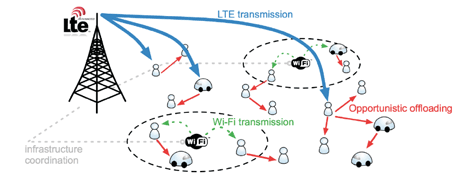
\includegraphics[width=3in]{pics/ONs.png}
  \caption{Scenariul descărcării oportuniste}
  \label{fig:pic1}
\end{figure}
Ideea de bază constă în faptul că offloading-ul poate fi mult mai benefic în momentul în care un număr mare de noduri aflate în aceeași comunitate sau în comunități apropiate, fiind situate într-o compactă arie fizică, doresc să descarce aproape aceași informație în aproximativ același timp de la serverele centrale. Așadar, fiecare nod are posibilitatea de a primi informația dorită de la un nod cu care s-a întâlnit, care la rândul lui are informația fie de la alte noduri cu care a avut contact în comunitate, fie folosim rețeaua celulară.(ex. stadionul de fotbal)

În literatura de specialitate întâlnim numeroși algoritmi de rutare în rețele oportuniste, fiecare având avantaje și dezavantaje în funcție de caracteristicile rețelei. Majoritatea mecanismelor de a împărți date în rețelele oportuniste se bazează pe distribuția de date Epidemic, care presupune că în momentul în care două noduri se întâlnesc primul nod își transferă datele la nodul întâlnit.  Acesta din urmă le salvează pe cele pe care nu le deține deja salvate dintr-o întâlnire anterioară și îi transferă și el propriile date. Punctele tari ale acestui mecanism sunt reprezentate de faptul că numărul mare de copii din rețea reduce întârzierea de transmitere, oferă o rată maximă mesajelor generate de a ajunge la destinație, fiind în același timp și cel mai simplu de implementat. În schimb punctele slabe sunt reprezentate de nevoia ca nodurile să aibă o memorie nelimitată, cât și de inundarea? rețelei cu mesaje, ceea ce face că în această formă să fie practic imposibil de folosit în viața reală. Așadar, implementările acestei distribuții au folosit un număr limitat de mesaje pentru a putea preveni aglomerarea rețelei, dar și din cauza faptului că toate nodurile vor avea o memorie limitată. Spray and Wait~\cite{SprayAndWait} este un astfel de algoritm care deși limitează numărul de mesaje care pot fi trimise in rețea, păstrează o rată ridicată de reușită. Acest algoritm presupune permiterea unui număr limitat si predefinit de copii pe care un mesaj al unui anumit nod le poate avea în rețea. Astfel identificăm două faze, si anume faza de împrăștiere și faza de așteptare. În prima fază fiecare nod primește câte o copie a mesajului în ordinea în care sunt întâlnite, până se ating numărul de copii permise, apoi începe faza a doua, de așteptare, în care nodurile ce dețin copia mesajului așteaptă întâlnirea nodul destinație, deoarece doar lui mai pot să il transfere. Deși această versiune nu garantează o rată maximă de reușită, valoarea ei este una ridicată ținând cont că rezolvă și o problemă importantă, anume congestia rețelei. 

\section{Mobile Edge Computing}
În zilele noastre, utilizatorii de dispozitive mobile inteligente sunt dependenți de execuția și stocarea unor operații intensive pe acestea. Majoritatea serviciilor precum: Facebook, Amazon, Google, dar și conținutul de pe Youtube sau Twitter este salvat in cloud, astfel pentru a realiza interacțiunea dorită cu aceste aplicații informațiile cerute de utilizator trebuie descărcate local. Pentru a face acest lucru cât mai optim trebuie să aducem cloudul cât mai aproape de utilizator și de marginea rețelei, altfel soluțiile sunt mult mai scumpe și dificile. Pentru aceste cerințe ale utilizatorilor se introduce idee de Mobile Edge Computing(MEC) care presupune că resursele necesare stocării, calculării, cât și rețelisticii sunt integrate alături de stațiile de bază, mult mai aproape de utilizatorul final. Așadar aplicațiile ce presupun un calcul intensiv și o latență semnificativă pot fi găzduite la marginea rețelei, datele lor fiind propagate mult mai ușor și rapid către destinatar, acest aspect fiind evidențiat și in Figura~\ref{fig:pic0}~\footnote{Această imagine a fost preluată de pe site-ul \cite{MECPicture} }.
\begin{figure}[th]
\centering
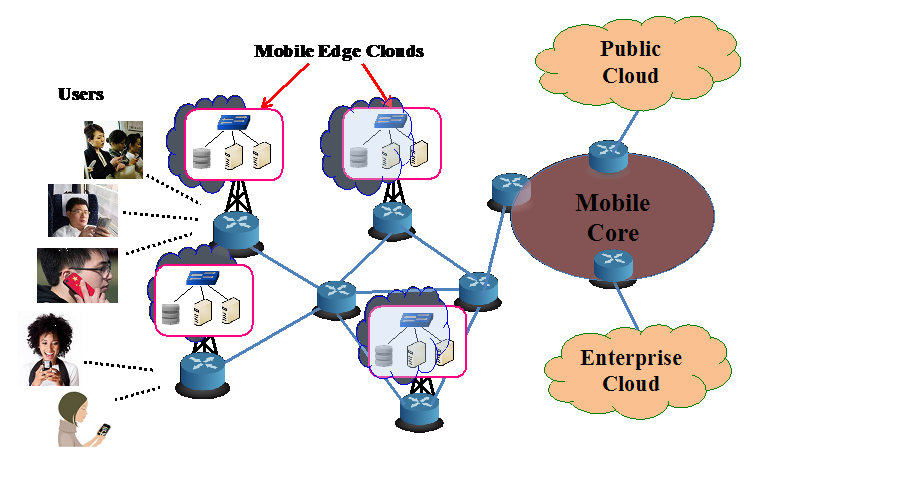
\includegraphics[width=3in]{pics/mobile-edge-computing.jpg}
  \caption{\emph{Exemplificarea cloud-urilor formate la marginea rețelei}}
  \label{fig:pic0}
\end{figure}

Într-o altă paradigmă numită Internet Of Things procesarea datelor este făcută de dispozitive aflate în aceeași rețea cu mașinăriile care au generat datele, astfel cu mecanisme de caching datele de pe cloud sunt accesate cu o latență scăzută datorită faptului că ele sunt transferate mai aproape de punctul de interes grație rețelelor Content Delivery(CDNs). Mobile Edge Computing-ul\cite{MecSurvey} sugerează folosirea unei scălari a comunicației pe orizontală în detrimentul unei scalări verticale de infrastructură cloud în momentul în care modelul de date din cloud nu mai este fezabil. Această paradigmă oferă un mediu de calcul extrem de distribuit folosit atât pentru dezvoltarea de aplicații și servicii, cât și pentru stocarea și procesarea datelor cât mai aproape de dispozitivele mobile. O aplicație poate fi divizată în mai multe sub-taskuri și împărțită prin rețea astfel o parte din sub-taskuri să fie rezolvate într-un cloud format local, la marginea rețelei, fie transmis la cloudul regional atât timp cât latența și precizia rămân în limitele dorite.

Așa cum reiese și din cele prezentate mai sus, conceptul de MEC se concentrează pe anumite metrici importante, cum ar fi latența și lățimea de bandă ridicată necesară comunicării. Aceste aspecte se îmbunătățesc prin limitarea transferului de date la serverele MEC, decât la serverele centralizate care prezintă un cost ridicat de întârziere. De asemenea, consumul de putere este o importantă grijă, astfel taskurile intens computaționale sunt mutate de la resursele dispozitivului utilizatorului către sisteme externe cu resurse puternice. Toate aceste îmbunătățiri vin cu un cost ridicat de implementare, deoarece atât crearea infrastructurii pentru MEC, cât și mentenanța ei necesită un important buget. 

.....
\section{Drop Computing}
Paradigma de Drop Computing\cite{DC} presupune descentralizarea computing-ului peste rețele cu mai multe nivele, prin combinarea tehnologiilor cloud si wireless peste o mulțime socială formată din dispozitive mobile si de margine. Astfel, în loc ca fiecare request de date sau calcule să fie direcționat către cloud, Drop Computing folosește dispozitivele din proximitate pentru un acces mai rapid si eficient. Nevoia pentru această paradigmă vine din insuficiența modelului cloud clasic care deja devine nepotrivit în marea ascensiune a scenariului Internet of Things. Când un număr mare de dispozitive comunică între ele, toate sunt nevoite să trimită request-uri către cloud, să aștepte răspunsul si apoi să-l proceseze, chiar dacă aceste dispozitive sunt chiar și la câțiva pași distanța.

Ca o concluzie principalul scop al acestei opțiuni este să minimizeze consumul de energie, să reducă costurile operaționale și chiar să măreasca performanțele rețelelor mobile comparativ cu celelalte modele, atât ca timp, cât și ca nivel de siguranță.
	
\begin{figure}[th]
\centering
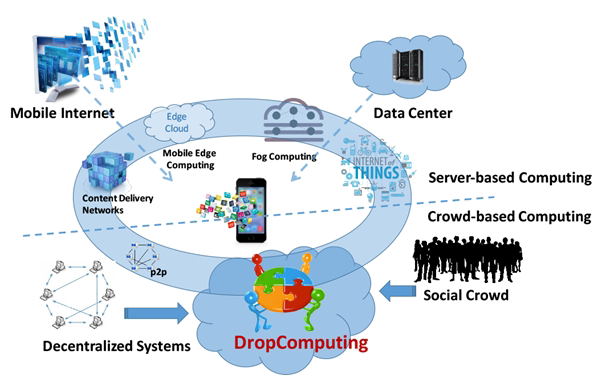
\includegraphics[width=3in]{pics/dropComputing.png}
  \caption{Viziunea Drop Computing}
  \label{fig:pic2}
\end{figure}

Așa cum sugerează și Figura~\ref{fig:pic2}\footnote{Aceasta imagine a fost preluată din articolul\cite{DC}} de mai sus, viziunea Drop Computing este de a extinde până la extrem modelul edge cloud, în loc de a avea dispozitive de margine fixe care să facă legătura cu cloud-ul, avem un cloud de margine. Acesta fiind o rețea dinamică ad hoc formată din dispozitive mobile aflate într-un anumit perimetru. Principala noutate a acestei paradigme provine din faptul că mobilitatea nodurilor(a dispozitivelor mobile) este văzută ca o caracteristică(feature) și nu ca o problemă ca până acum. Astfel conexiunile sociale între dispozitive, mai exact între persoanele purtătoare și posesoare de dispozitive mobile, sunt utilizate pentru a calcula atât nivelul de încredere, cât si nivelul de reușită atunci când se folosesc resursele altor noduri. Concluzionând, distribuirea si salvarea datelor de către nodurile din rețea care au o importantă probabilitate de întâlnire cu dispozitivele ce necesită acele informații reprezintă un important beneficiu prin faptul că datele sunt aduse mult mai aproape de utilizator, interacțiunea cu cloud-ul nemaifiind atât de intensă.

\section{MobEmu}
MobEmu~\cite{MobEmuArticle} este un simulator de rețele oportuniste care poate repeta o urmă(trace, comportament) care este fie rezultatul unei măsuratori din viața reală, fie este rezultat/ă în urma rulării unui model sintetic de mobilitate. Acestor date urmează să li se aplice un algoritm de rutare și diseminare creat de utilizator.
În timp ce modelul fizic?? presupune analiza unui experiment în care participanții poartă diferite dispozitive care înregistrează interacțiunile dintre ei ca moment de timp și durata contactului, modelele sintetice sunt modele matematice care pot simula diferite comportamente ale nodurilor. Dacă Shortest Path Map-Based model~\cite{ShortestPathMapBased} alege viteza de deplasare a nodurilor random, urmatoarea poziție o alege random dintr-o listă de puncte valide de pe hartă. În continuare, utilizează un algoritm de calcul pentru cel mai scurt drum dintre două puncte precum Dijkstra și găsește cel mai scurt drum până la destinație, ținând cont și de anumite direcții valide(e.g care să nu treacă prin ziduri). 
Pentru a putea rula și testa soluțiile care au stat la baza acestei lucrări am folosit MobEmu, un simulator scris in Java a cărui funcționalitate o voi descrie in continuare. 

În primul rând, acest framework oferă posibilitatea alegerii între mai multe tipuri de parsere: de la cele care simuleaza modelele sintetice până la cele care analizează datele colectate de diferite dispozitive din facultate. La fiecare moment de timp, de când s-a măsurat trace-ul si până când s-a terminat, se verifică orice contact care apare între cel puțin două noduri. În momentul în care a avut loc un contact se poate folosi un algoritm de rutare și diseminare, unul dorit și implementat de utilizator. 
(as zice aici un ``in al doilea rand'' )Alături de acestea, MobEmu permite ca utilizatorul să controleze la fiecare moment de timp generarea de mesaje a unui nod către alte noduri, dar și numărul lor, prioritatea, Time-To-Live, numărul total de copii pe care îl permite in rețea. Totodată, simulatorul calculează comunitatea din care face parte fiecare nod utilizând algoritmul k-CLIQUE sau alți algoritmi care utilizează detecția bazată pe euristici cognitive. 
În final se oferă statistici cu privire la numărul de mesaje care au ajuns la destinație, timpul în care acestea s-au propagat prin rețea, numărul de comunități create, latența și costul transportului, toate acestea fiind influențate de anumite setări pe care le poate face utilizatorul precum memoria fiecărui nod, viteza cu care mesajele se pot transmite, dar și nivelul de altruism al nodurilor.

Pe lângă acest simulator, mai există și altele care se comportă în mod asemănator, cel mai cunoscut fiind ONE(Opportunistic Network Environment)~\cite{OneArticle} disponibil tot in java și care modelează mobilitatea nodurilor, contactele inter noduri, dar și rutarea pachetelor. Fiecare nod este reprezentat de un modul principal care la rândul lui se poate conecta la diferite submodule precum: energia consumată, mobilitatea, memoria, descriind astfel capabilitățile și atributele nodului ONE. Decizia de a folosi MobEmu a venit în urma unor avantaje pe care acesta le oferă, și anume: suport pentru detectarea comunităților de noduri, folosirea conexiunilor din rețelele sociale, modelarea altruismului, permițând în același timp și simularea unor comportamente în care mesajele nu sunt propagate către o singură destinație. Aceste avantaje consider că se mapează mult mai bine pe situațiile reale, în care posesorii dispozitivelor inteligente pot respecta un anumit pattern de mobilitate sau de conținut cerut în funcție de relațiile sociale, dar și de comunitatea din care fac parte in acel moment.  


\section{Metode de realizare a consistenței datelor}

\subsection{Disponibilitatea datelor și nevoia de replicare a datelor}
Majoritatea paradigmelor descrise anterior sugerează ideea de a avea conexiune oriunde ne-am afla și la orice moment de timp. Acest lucru devine o necesitate în anumite situații critice precum dezastrele naturale sau acțiuni militare, atunci când infrastructura de comunicație are de suferit. Disponibilitatea datelor se referă la reușirea transmiterii datelor de la sursă către destinație într-un interval de timp rezonabil, optim. Replicarea datelor este o tehnică de asigurare a disponibilității datelor prin realizarea de copii ale datelor și propagarea lor prin diferite noduri din rețea. Astfel, prin această tehnică se reușește un schimb mai bun de date datorită faptului că timpul de răspuns la cererile multiple poate fi îmbunătățit prin distribuirea procesării cererilor pe mai multe noduri. În momentul în care în rețea datele sunt prezente doar la un singur nod acest lucru nu este benefit, putând chiar avea rezultate mai slabe, dar prin copierea datelor în mai multe noduri acest procedeu reușește să evite o supraîncărcare a rutelor de comunicație către un unic nod. 
\subsection{Problemele algoritmilor de replicare}
Replicarea datelor reduce numărul de întârzieri al cererilor înregistrate, cu toate acestea folosirea acestui mecanism poate duce și la o durată mai mare a anumitor întârzieri. Acest lucru se poate întâmpla datorită faptului că disponibilitatea datelor scade în momentul în care multe noduri aflate într-o mică proximitate duplică același set de date, în timp ce alte date nu sunt replicate de niciun nod. O soluție la această problemă ar putea fi duplicarea datelor în noduri care au un număr setat de hopuri între ele, nu se întâlnesc într-o anumită vecinătate. Această soluție simplă prezintă anumite dezavantaje, iar cel mai important este acela că se poate înregistra un timp mai mare de întârziere pentru o anumită desfășurare a cererilor, adică ceea ce trebuia să repare în totalitate, rezolvă doar parțial. Problema apare datorită faptului că într-o anumită proximitate nu vom putea duplica datele care au procentaj ridicat de accesare. Din această cauză, dar și datorită mobilității nodurilor o schemă statică de alocare a duplicatelor într-o topologie dinamică nu este posibilă.
\subsection{Predicția mobilității nodurilor}
Mobilitatea nodurilor este principala îngrijorare când vine vorba despre un algoritm de replicare a datelor, deoarece este considerată principala cauză a partiționării rețelei. Așadar, dacă un nod(adică posesorul unui dispozitiv mobil) se deplasează în afara zonei de acțiune pentru o anumită vecinatate, nu va mai putea oferi servicii nodurilor din perimetrul ce tocmai l-a părăsit. Se observă că se poate păstra disponibilitatea datelor în acea proximitate la același nivel dacă se poate prezice o eventuală deplasare a nodurilor, având ca scop duplicarea datelor de interes de la acele noduri la cele mai apropiate care sunt în continuare în acea suprafață. Pushpalatha. M et al\cite{DesignDRA} fac anumite presupuneri înainte de a expune un algoritm de predicție și anume: nodurile din rețea sunt simetric conectate, rețeaua nu este partiționată și fiecare nod poate măsura intensitatea semnalului pe care îl primește. Ecuația de transmisie Friss\cite{Friss} este folosită pentru a calcula intensitea semnalului recepționat având următoarea formă : 
\begin{equation}
P_{r} = P_{t} * A_{r} * A_{t} * \lambda^2 / (4 * \pi * d)^2
\end{equation}
unde: 
$
P_{r}		-	\;puterea\; la\; receptor;\quad
P_{t}  	- \;puterea\; la\; transmisie;\quad
A_{r}   - \;amplificarea\; antenei\; la\; recepție;\\
A_{t} 	- \;amplificarea\; antenei\; la\; transmisie;\quad
\lambda - \;lungimea\; de\; unda;\quad
d 			- \;distanța\; dintre\; noduri.\\
$
Prin urmare, derivând ecuația de mai sus în cele două puncte se estimează valoarea distanței ca fiind egală cu:
\begin{equation}
d = k / \sqrt{Pr}
\label{eq:}
\end{equation}
unde: 
$
k -\;constanta\quad
P_{r} -\;puterea\; la\; receptor \\
$
Fiecare nod trimite în mod periodic un mesaj de tip Hello, estimând distanța până la respectivul nod, iar pentru a estima mobilitatea unui nod se măsoară puterea semnalului dintre două mesaje Hello succesive. Apoi se estimează distanța dintre două noduri la două momente diferite de timp comparându-se cu o valoarea setată între distanța minimă de transmisie și distanța minimă de transmisie. Dacă diferența estimată este aproape de 0 atunci nodurile nu se vor mișca, dar dacă mai mare sau egală cu valoarea de referință se începe procesul de căutare a unor noduri potrivite pentru a reține date replicate în nodul care a fost prezis că va parăsi zona curentă de transmisie. Totodată ținând cont de necesitățile acestor tipuri de rețele și anume o latență cât mai mică și o încărcare mică a rutelor de comunicație, acest algoritm este destul de costisitor și nepotrivit, datorită faptului că acele mesaje periodice de Hello inundă rețeaua, dar și pentru că presupunerile de la început sugerează un comportament greu de mapat cu situațiile din viața reală, unde nu vom găsi doar noduri simetric conectate.

\subsection{Consistența datelor}
În rețelele mobile prezentate anterior, mobilitatea nodurilor creează partiționări frecvente ale rețelei, astfel o organizare(management) a consistenței datelor devine o problemă crucială. Takahiro Hara et al. ~\cite{hara2009consistency} prezintă diferite condiții de consistență ale datelor replicate în MANET, clasificând nivelurile de consistență în funcție de cerințele aplicațiilor. În această lucrare se presupune existența unui mediu în care fiecare dispozitiv poate accesa datele din alte stații replicându-le astfel în propriul spațiu de memorie. Rețeaua este divizată în mai multe regiuni și consistența datelor replicate este realizată în funcție de regiune. Cazurile care sunt prezentate în această lucrare au la bază două tipuri de dispozitive din cadrul rețelei: unul cu caracteristici speciale, denumit proxy, care fie au memorie nelimitată, fie cunosc cum sunt împărțite replicile în rețea,  celelalte fiind dispozitive simple ce își cunosc doar propriile replici. Nivelurile de consistență prezentate sunt caracterizate de: consistență globală, consistență bazată pe locație, pe timp, sau pe stație, iar ca rezultat general se afirmă că este mult mai benefic, în termeni de rată de succes și încărcare a traficului, alegerea unui protocol de consistență locală în detrimentul unei consistenței globale.(Protocolul 5.3.1 - e mult de scris nu stiu cum sa rezum)
Nithiyalakshmi et al.\cite{nithiyalakshmi2014data} propun tehnici distribuite de replicare a datelor pentru a echilibra compromisurilor dintre întârzierea interogărilor și disponibilitatea datelor. Metoda One-to-One Optimization(OTOO) folosește fiecare nod mobil care colaborează doar cu nodul vecin pentru a decide ce informație va găzdui. Astfel fiecare nod calculează o valoare a frecvenței accesului combinat la informația respectivă, salvând datele în ordinea ascendentă a acestor valori. Tehnica de replicare compune elementul de date replicat cu privire la frecvența de acces al elementelor de date, menținându-se astfel coerența datelor.

Pentru a menține eficient și sigur coerența cache\cite{knaesel2009high} în cadrul dispozitivelor mobile sunt folosite două tehnici în mod preponderent: notificarea privind o înregistrare invalidă, sau notificarea unei înregistrări valide. În timp ce prima tehnică este folosită când mai puțin de 50\% din datele de pe serverul staționar au fost schimbate, a doua tehnică se folosește pentru a reduce cantitatea de date transferate prin rețeaua wireless în momentul în care mai mult de 50\% din datele de pe server au suferit modificări. În prezent datele vin de la server, dar pot veni și de la alți clienți,dispozitive care se comportă ca un server. Pe măsură ce se folosește o abordare pesimistă, serverele neștiind ce date sunt stocate pe dispozitivele mobile, toate datele solicitate vor fi transmise prin rețea. Așadar se folosește un timestamp protocol pentru a asigura consistența și consecvența datelor salvate local, putând spune cu ajutorul valorii timestampului dacă data primită este mai nouă sau mai veche față de copia deja deținută. Una dintre preocupări și provocări în cadrul unui sistem distribuit este sincronizarea și menținerea unor generatoare de timestamp globale. Folosind această tehnică, sincronizarea ceasurile generatorilor de timestamp se poate realiza folosind Network Time Protocol(NTP), un protocol disponibil în rețeaua TCP/IP, al cărui rezultat garantează un nivel ridicat de consistență a datelor updatate.

Așa din reiese și din cele prezentate anterior, consistența datelor în aceste rețele este privită diferit față de ceea ce voi prezenta în această teză. Termenul de consistență este folosit în situațiile în care datele suferă anumite modificări, scrieri și se pune problema renunțării la toate replicările existente ale acelor date pentru a nu genera rezultate nedorite influențate de folosirea unei versiuni anterioare a acelor date. Totuși, consistența datelor trebuie realizată la orice moment de timp și în orice împrejurare ținând cont de toate posibilitățile de incoerență, iar modificarea intenționată a unor informații este poate cea mai frecventă alterare a coerenței datelor. Ținând cont de caracteristicile acestui tip de rețele mobile consider că această abordare legată de consistența datelor are aplicabilitate în numeroase scenarii din viața reală.  (Aici: teste cu privire la gradul de corupere, cat de multe date se corup in medie intr-o retea din cauze intentionate)  


!!!Cerinta - Sunt descrise tehnologii alternative. Sunt analizate cantitativ și calitativ, folosite benchmarkuri și teste efectuate de student. Analiza este rezumată prin tabele și grafice.!!!

!!!legat de ONE!!!
As putea pune in comparatie aici drop computing fata de versiunea standard de folosire a cloudului, cu scenariile dezbatute in paperul DC??
\ambele În încheierea acestui capitol se dorește descrierea tehnologiilor folosite în lucrare, cu alternative și cu argumente convingătoare calitative și cantitative.  


Criterii pentru calificativul \textit{Ne\textit{Satisfăcător}}: 
\begin{itemize}
	\item \dezvoltare Sunt analizate superficial câteva produse de pe piață; 
	\item \cercetare analiza literaturii limitata la grupuri de cercetare din România;
	\item \ambele Sunt descrise tehnologiile folosite în lucrare. 
\end{itemize}

Criterii pentru calificativul \textit{Satisfăcător}:
\begin{itemize}
	\item \dezvoltare Există un interviu, un client, analiza cerințelor este elaborată pe baza interviului.
	\item \cercetare analiza literaturii de specialitate din lume, fără poziționarea precisă a lucrării în peisajului domeniului studiat;
	\item \ambele Sunt descrise câteva tehnologii alternative pentru fiecare din tehnologiile folosite în lucrare. Există o argumentare referitoare la alegere.
\end{itemize}

Criterii pentru calificativul \textit{Bine}:
\begin{itemize}
	\item \dezvoltare Proces iterativ pe baza unor interviuri cu mai mulți clienți, dezvoltare MVP, reevaluare cerințe;
	\item \cercetare analiza literaturii de specialitate din lume, cu poziționarea precisă a lucrării în peisajul actual al domeniului studiat; 
	\item \ambele Sunt descrise tehnologii alternative. Sunt analizate cantitativ și calitativ, folosite benchmarkuri și teste efectuate de student. Analiza este rezumată prin tabele și grafice.
\end{itemize}

\section{Indicații formatare figuri}

Figurile utilizate în document vor fi centrate și numerotate (de exemplu Figura~\ref{fig:pic1}). 
Orice figură ce nu este realizată de către autorul lucrării va fi în mod obligatoriu citată fie la final (de exemplu Figura ~\ref{fig:pic2} este preluată din documentul \cite{}), fie cel puțin într-o notă de subsol (a se vedea Figura~\ref{fig:pic2}). Orice figură ce depășește ca dimensiune 50\% dintr-o pagină, va fi mutată la anexe. Toate figurile din cadrul tezei vor fi referite în text. Exemplu: Figura~\ref{fig:pic1} prezintă o schemă de principiu pentru un amplificator inversor cu AO. 

\begin{figure}[th]
\centering
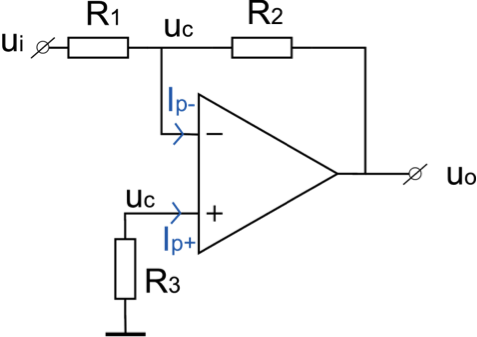
\includegraphics{pics/Pic1.png}
  \caption{Amplificator inversor}
  \label{fig:pic1}
\end{figure}

\newpage

\begin{figure}[th]
\centering
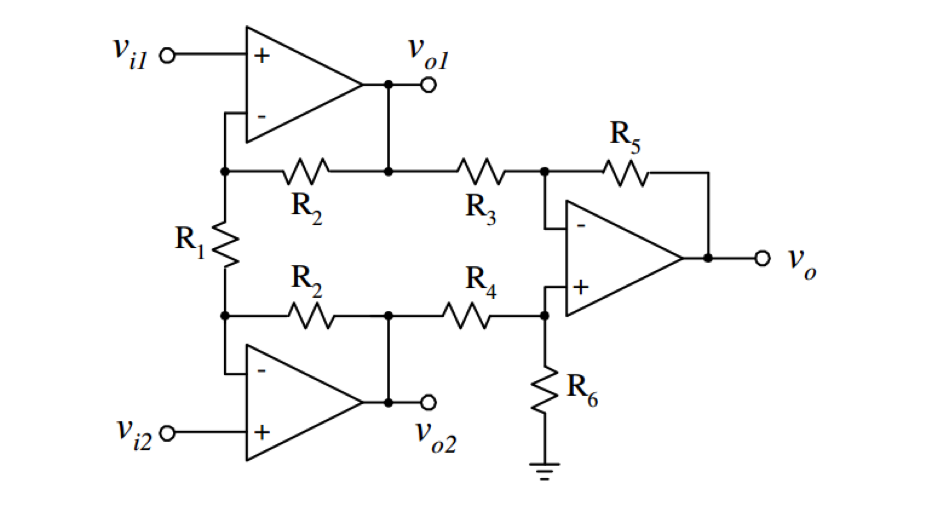
\includegraphics{pics/Pic2.png}
  \caption[Amplificator de instrumentație cu 3 AO-uri]{Amplificator de instrumentație cu 3 AO-uri\protect\footnotemark}
  \label{fig:pic2}
\end{figure}
\footnotetext{© http://www.ece.tamu.edu/sspalermo/ecen3205/Secton\%201III.pdf}

\chapter{Soluția Propusă}
Capitolul conține o privire de ansamblu a soluției ce rezolvă problema, prin prezentarea structurii / arhitecturii acesteia. În funcție de tipul lucrării acest capitol poate conține diagrame (clase, distribuție, workflow, entitate-relație), demonstrații de corectitudine pentru algoritmii propuși de autor, abordări teoretice (modelare matematică), structura hardware, arhitectura aplicației.


Criterii pentru calificativul \textit{Ne\textit{Satisfăcător}}: 
\begin{itemize}
	\item	Descriere în limbaj natural.
\end{itemize}

Criterii pentru calificativul \textit{Satisfăcător}: 
\begin{itemize}
	\item	Descriere + diagrame de baze de date, workflow, clase, algoritmi. 
\end{itemize}

Criterii pentru calificativul \textit{Bine}: 
\begin{itemize}
	\item 	Descriere + diagrame de baze de date, workflow, clase, algoritmi + descrierea unui proces prin care s-a realizat arhitectura/structura soluției.
\end{itemize}

\section{Indicații formatare formule}
Formulele matematice utilizate în document vor fi centrate în pagină și numerotate. 

\begin{equation}
(x+a)^n = \sum_{k=0}^{n}\left(\begin{array}{c}n\\k\\\end{array}\right)x^ka^{n-k}
\end{equation}

\begin{equation}
f(x) = a_0 + \sum_{n=1}^{\infty}\left(a_n \cos\frac{n\pi x}{L} + b_n\sin\frac{n\pi x}{L}\right)
\end{equation}



\chapter{Detalii de implementare}
În plus fata de capitolul precedent acesta conține elemente specifice ale rezolvării problemei care au presupus dificultăți deosebite din punct de vedere tehnic. Pot fi incluse configurații, secvențe de cod, pseudo-cod, implementări ale unor algoritmi, analize ale unor date, scripturi de testare. De asemenea, poate fi detaliat modul în care au fost utilizate tehnologiile introduse in capitolul 3.


Criterii pentru calificativul \textit{Ne\textit{Satisfăcător}}: 
\begin{itemize}
	\item	Sunt prezentate pe scurt scheme și pseudo-cod.
\end{itemize}
Criterii pentru calificativul \textit{Satisfăcător}: 
\begin{itemize}
	\item	Descriere sumara a implementării, prezentarea unor secvențe nerelevante de cod, scheme, etc. 
\end{itemize}
Criterii pentru calificativul \textit{Bine}: 
\begin{itemize}
	\item	Descrierea detaliată a algoritmilor/structurilor utilizați; Prezentarea etapizată a dezvoltării, inclusiv cu dificultăți de implementare întâmpinate, soluții descoperite; (dacă este cazul) demonstrarea corectitudinii algoritmilor utilizați. 
\end{itemize}

\section{Indicații formatare tabele}
Se recomandă utilizarea tabelelor de forma celui de mai jos.  Font size :  9. 
Orice tabel prezent în teză va fi referit în text; exemplu: a se vedea Tabel~\ref{tab:criterii}.

\begin{table}[th]\small\linespread{1}
\caption{Sumarizare criterii}
\label{tab:criterii}
\begin{tabular}{l >{\raggedright\arraybackslash}p{8cm} >{\raggedright\arraybackslash}p{4cm}}
\textbf{Calificativ} & \textbf{Criteriu} & \textbf{Observații} \\\hline
\textbf{Nesatisfacator} & Sunt prezentate pe scurt scheme și pseudo-cod & \\\hline
\textbf{Satisfacator} &Descriere sumara a implementării, prezentarea unor secvențe nerelevante de cod, scheme, etc.& \\
\hline
\textbf{\textit{Bine}} &Descrierea detaliată a algoritmilor/structurilor utilizați; Prezentarea etapizată a dezvoltării, inclusiv cu dificultăți de implementare întâmpinate, soluții descoperite; (dacă este cazul) demonstrarea corectitudinii algoritmilor utilizați. & Pot fi incluse configurații, secvente de cod, pseudo-cod, implementări ale unor algoritmi, analize ale unor date, scripturi de testare. \\
\hline
\end{tabular}
\end{table}


\chapter{Evaluare}
Acest capitol trebuie să răspundă, în principiu, la 2 întrebări și să se încheie cu o discuție a rezultatelor obținute. Cele doua întrebări la care trebuie sa se răspundă sunt:
\begin{enumerate}
	\item  \textbf{Merge corect?} (Conform specificațiilor extrase în capitolul 2); 
Evaluarea dacă merge corect se face pe baza cerințelor identificate în capitolele anterioare. 

	\item Cât de \textit{Bine} merge / cum se compară cu soluțiile existente? (pe baza unor metrici clare). 
Evaluarea cât de \textit{Bine} merge trebuie să fie bazată pe procente, timpi, cantitate, numere, \textbf{comparativ cu soluțiile prezentate în capitolul 3}. Poate fi vorba de performanță, overhead, resurse consumate, scalabilitate etc. 
\end{enumerate}

În realizarea discuției, se vor utiliza tabele cu procente, rezultate numerice și grafice. În mod obișnuit, aici se fac comparații și teste comparative cu alte proiecte similare (dacă există) și se extrag puncte tari și puncte slabe. Se ține cont de avantajele menționate și se demonstrează viabilitatea abordării / aplicației, de dorit prin comparație cu alte abordări (dacă acest lucru este posibil). Cuvântul cheie la evaluare este ``metrică'': trebuie să aveți noțiuni măsurabile și cuantificabile. În cadrul procesului de evaluare, explicați datele, tabelele și graficele pe care le prezentați și insistați pe relevanța lor, în următorul stil: ``este de preferat ... deoarece …''; explicați cititorului nu doar datele ci și semnificația lor și cum sunt acestea interpretate. Din această interpretare trebuie să rezulte poziționarea proiectului vostru printre alternativele existente, precum și cum poate fi acesta îmbunătățit în continuare.

Criterii pentru calificativul \textit{Ne\textit{Satisfăcător}}: 
\begin{itemize}
	\item Aplicația este testată dar rulează pe calculatorul studentului, nu există posibilități de testare, nu a fost validată cu clienți / utilizatori;
	\item Nu au fost realizate comparații cu alte sisteme similare.
\end{itemize}

Criterii pentru calificativul \textit{Satisfăcător}: 
\begin{itemize}
	\item \dezvoltare  Există teste unitare și de integrare, există o strategie de punere în funcțiune (deployment), există validare minimală cu clienții / utilizatorii.
	\item \cercetare Principalele componente și soluția în ansamblu au fost evaluate din punct de vedere al performanței, însă nu sunt folosite seturi de date standard, există unele erori de interpretare a datelor.
	\item \ambele Discuție minimală asupra relevanței rezultatelor prezentate, comparație minimală cu alte sisteme similare.
\end{itemize}

Criterii pentru calificativul \textit{Bine}: 
\begin{itemize}
	\item \dezvoltare Teste unitare și de integrare, instrumente de punere in funcțiune (deployment) utilizate și care arată lucru constant de-a lungul semestrului, lucrare validată cu clienții / utilizatorii, produs în producție.
	\item \cercetare Componentele și soluția în ansamblu au fost evaluate din punct de vedere al performanței, folosind seturi de date standard și cu o interpretare corectă a rezultatelor.
	\item \ambele Discuție cu prezentarea calitativă și cantitativă a rezultatelor, precum și a relevanței acestor rezultate printr-o comparație complexă cu alte sisteme similare.
\end{itemize}

\chapter{Concluzii}
În acest capitol este sumarizat întreg proiectul, de la obiective, la implementare, si la relevanta rezultatelor obținute. În finalul capitolului poate exista o subsecțiune de ``Dezvoltări ulterioare''.

Criterii pentru calificativul \textit{Ne\textit{Satisfăcător}}: 
\begin{itemize}
	\item	Concluziile nu sunt corelate cu conținutul lucrării;
\end{itemize}

Criterii pentru calificativul \textit{Satisfăcător}: 
\begin{itemize}
	\item	Concluziile sunt corelate cu conținutul lucrării, însă nu se oferă o imagine asupra calității și relevantei rezultatelor obținute;
\end{itemize}

Criterii pentru calificativul \textit{Bine}: 
\begin{itemize}
	\item	Concluziile sunt corelate cu conținutul lucrării, și se oferă o imagine precisa asupra relevantei și calității rezultatelor obținute în cadrul proiectului. 
\end{itemize}

\chapter{Bibliografie}
% * <marios.choudary@gmail.com> 2018-02-28T12:07:48.730Z:
% 
% > BIBLIOGRAFIE
% Am adaugat un paragraf cu cateva detalii despre folosirea citarilor bibliografice in Latex, despre folosirea lui "\cite" si despre posibilitatea folosirii bibliografiei si direct in fisierul Latex.
% 
% ^.

\begin{itemize}
	\item 	NU utilizați referințe la Wikipedia sau alte surse fără autor asumat.
	\item 	Pentru referințe la articole relevante accesibile în web (descrise prin URL) se va nota la bibliografie și data accesării.
	\item 	Mai multe detalii despre citarea referințelor din internet se pot regăsi la:
	\begin{itemize}
		\item	\url{http://www.writinghelp-central.com/apa-citation-internet.html}
		\item	\url{http://www.webliminal.com/search/search-web13.html}
	\end{itemize}
	\item 	Note de subsol se utilizează dacă referiți un link mai puțin semnificativ o singură dată; Dacă nota este citată de mai multe ori, atunci utilizați o referință bibliografică.
	\item 	Dacă o imagine este introdusă în text și nu este realizată de către autorul lucrării, trebuie citată sursa ei (ca notă de subsol sau referință - este de preferat utilizarea unei note de subsol).
	\item 	Referințele se pun direct legate de text (de exemplu ``KVM [1] uses'', ``as stated by Popescu and Ionescu [12]'', etc.). Nu este recomandat să folosiți formulări de tipul ``[1] uses'', ``as stated in [12]'', ``as described in [11]'' etc..
	\item 	Afirmațiile de forma ``are numerous'', ``have grown exponentially'', ``are among the most used'', ``are an important topic'' trebuie să fie acoperite cu citări, date concrete si analize comparative.
	\begin{itemize}
		\item	Mai ales în capitolele de introducere, ``state of the art'', ``related work'' sau ``background'' trebuie să vă argumentați afirmațiile prin citări. Fiți autocritici și gândiți-vă dacă afirmațiile au nevoie de citări, chiar și cele pe care le considerați evidente.
		\item	Cea mai mare parte dintre citări vor fi în capitolele de introducere ``state of the art'', ``related work'' sau ``background''.
	\end{itemize}
	\item 	Toate intrările bibliografice trebuie citate în text. Nu le adăugați pur și simplu la final.
	\item 	Nu copiați sau traduceți niciodată din surse de informație de orice tip (online, offline, cărți, etc.). Dacă totuși doriți să oferiți, prin excepție, un citat celebru - de maxim 1 frază- utilizați ghilimele și evident menționați sursa. .
	\item 	Dacă reformulați idei sau creați un paragraf rezumat al unor idei folosind cuvintele voastre, precizați cu citare (referință bibliografică) sau cu notă de subsol sursa sau sursele de unde ați preluat ideile.
\end{itemize}

Trebuie respectat un singur standard de trimiteri bibliografice (citare), dintre următoarele alternative:
\begin{itemize}
	\item APA (\url{http://pitt.libguides.com/c.php?g=12108\&p=64730})
	\item IEEE (\url{https://ieee-dataport.org/sites/default/files/analysis/27/IEEE\%20Citation\%20Guidelines.pdf}) 
	\item Harvard (\url{https://libweb.anglia.ac.uk/referencing/harvard.htm})
	\item Cu numerotarea referințelor în ordine alfabetică sau în ordinea apariției în text (de exemplu, stilul cu numere folosit de unele publicații ACM - \url{https://www.acm.org/publications/authors/reference-formatting}) 
\end{itemize}

În Latex este foarte ușor să folosiți referințe într-un mod corect și unitar, fie prin adăugarea unei secțiuni
\verb!\begin{thebibliography}!
(vezi la sfârșitul acestei secțiuni), fie printr-un fișier separat de tip bib, folosind comanda
\verb!\bibliography{}!,
așa cum procedăm mai jos prin folosirea fișierului ``bibliography.bib''. În orice caz, în Latex va trebui să folosiți comanda
\verb!\cite{}!
pentru a adăuga referințe, iar această comandă trebuie folosită direct în text, acolo unde vreți sa apară citația, ca în exemplele următoare:
\begin{itemize}
	\item Articol jurnal:
\end{itemize}

\textbf{Important}: în această secțiune de obicei apar doar intrările bibliografice (adică doar listarea referințelor). Citarea lor prin comanda cite și explicații legate de ele trebuie facute în secțiunile anterioare. Citarea de mai sus a fost facută aici doar pentru exemplificare.

% Asa se specifica folosirea unui fisier cu referinte bibliografice:
\bibliographystyle{plain}

\bibliography{bibliografie}



%% O alta varianta ar fi fost includerea de articole direct in acest fisier
%% in felul urmator:
%% \begin{thebibliography}{ABC}
%%
%% \bibitem{article}
%%  H. Baali, H. Djelouat, A. Amira and F. Bensaali,
%%  ``Empowering Technology Enabled Care Using IoT and Smart Devices:
%   A Review''. In: IEEE Sensors Journal, vol. 322 (10), pp. 891--921, 1905.
%%
%% (more \bibitem items here...)
%%
%% \end{thebibliography}

%% Daca vreti ca o sectiune sa inceapa pe o pagina noua, puteti forta acest lucru cu comanda "\newpage", ca mai jos:
\newpage

\chapter{Anexe}

Anexele sunt opționale.
Ce poate intra în anexe:
\begin{itemize}
\item	Exemplu de fișier de configurare sau compilare;
\item	Un tabel mai mare de o jumătate pagină;
\item	O figura mai mare mai mare de jumătate pagină;
\item	O secvență de cod sursa mai mare de jumătate pagină;
\item	Un set de capturi de ecran (``screenshot''-uri);
\item	Un exemplu de rulare a unor comenzi plus rezultatul (``output''-ul) acestora;
\item 	În anexe intră lucruri care ocupă mai mult de o pagină ce ar întrerupe firul natural de parcurgere al textului.
\end{itemize}

\end{document}